\documentclass[11pt,letterpaper]{article}

%\usepackage{fontspec}
%\usepackage[utf8]{inputenc}
\usepackage{textcomp,marvosym}
\usepackage{amsmath,amssymb}
\usepackage[normalem]{ulem}
\usepackage[left]{lineno}
\usepackage{changepage}
\usepackage{sidecap}
\usepackage{rotating}
\usepackage{color}
\usepackage{natbib}
\usepackage{setspace}
\usepackage{}
\usepackage{fancyhdr}
\usepackage{graphicx}
\usepackage{xspace}
\usepackage{threeparttable}
\usepackage{color,colortbl}
\usepackage{url}
%\usepackage[hidelinks]{hyperref}
\urlstyle{same}
\doublespacing

\raggedright
\textwidth = 6.5 in
\textheight = 8.25 in
\oddsidemargin = 0.0 in
\evensidemargin = 0.0 in
\topmargin = 0.0 in
\headheight = 0.0 in
\headsep = 0.5 in
\parskip = 0.1 in
\parindent = 0.1in

% Bold the 'Figure #' in the caption and separate it from the title/caption with a period
% Captions will be left justified
\usepackage[aboveskip=1pt,labelfont=bf,labelsep=period,justification=raggedright,singlelinecheck=off]{caption}

% Remove brackets from numbering in List of References
%\makeatletter
%\renewcommand{\@biblabel}[1]{\quad#1.}
%\makeatother

% Self defined commands
\newcommand{\degC}{$^{\circ}$C\xspace}
\newcommand{\dC}{$\delta^{13}$C\xspace}
\newcommand{\dO}{$\delta^{18}$O\xspace}
\newcommand{\SrSr}{$^{87}$Sr/$^{86}$Sr\xspace}
\newcommand{\permil}{\textperthousand\xspace}
\newcommand{\dsil}{$d$\xspace}

\setcounter{figure}{0}
\renewcommand{\thefigure}{DR\arabic{figure}}
\setcounter{table}{0}
\renewcommand{\thetable}{DR\arabic{table}}

\definecolor{Yellow}{rgb}{1,1,0.35}
%

\pagestyle{myheadings}
\pagestyle{fancy}
\fancyhf{}
\lhead{Park et al., in review for XXX}
\rhead{\thepage}

\begin{document}

\begin{flushleft}
{\Large \textbf{Data Repository for ``GEOCLIM Modern''}}
\\
Yuem Park\textsuperscript{1},
Nicholas L. Swanson-Hysell\textsuperscript{1},
Pierre Maffre\textsuperscript{2},
Yves Godd\'eris\textsuperscript{2}
\\
\bigskip
\textsuperscript{1} Department of Earth and Planetary Science, University of California, Berkeley, CA, USA
\\
\bigskip

\end{flushleft}

\linenumbers

These repository materials provide details on the model framework used in this study. Python code used for this study can be found at: \url{https://github.com/Swanson-Hysell-Group/XXX}.

\section*{Silicate Weathering Component}

\begin{SCfigure}[0.6][h!]
\begin{center}
	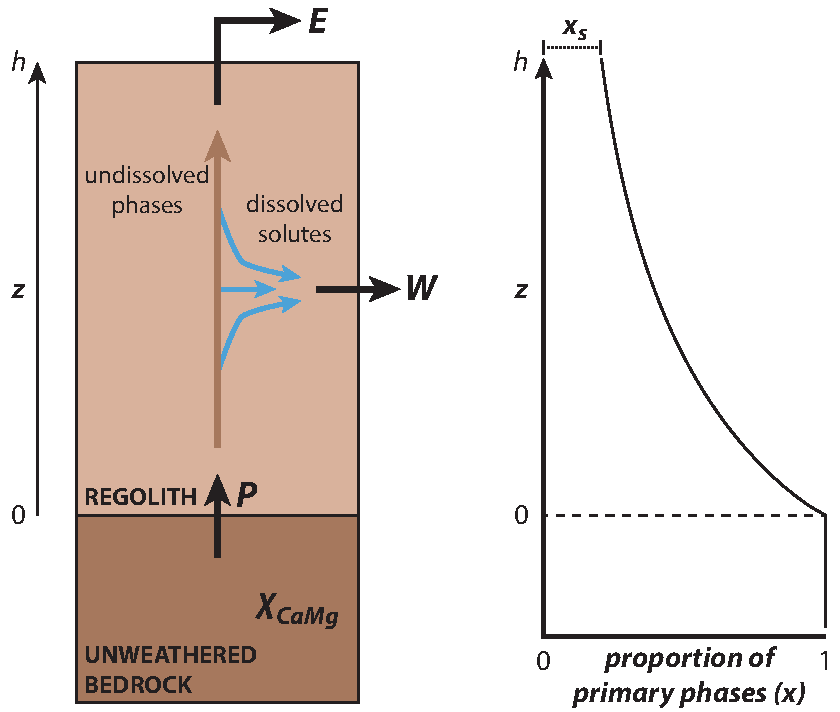
\includegraphics[width=0.6\textwidth]{../Figures/regolith_schematic.pdf}
	\caption{A schematic representation of the silicate weathering component of GEOCLIM in a single profile at steady-state. A rock particle leaves the unweathered bedrock with production rate $P$, and transits vertically through a regolith of height $h$. Regolith production and physical erosion ($E$) are equal at steady-state. As the particle transits upwards, some fraction of the primary phases ($x$) are chemically weathered ($W$) with the flux of Ca and Mg corresponding to that weathering rate multiplied by the concentration of Ca+Mg in unweathered bedrock ($\chi_{CaMg}$).}
	\label{fig:regolith_schematic}
\end{center}
\end{SCfigure}

The silicate weathering portion of the GEOCLIM model implements the model of \cite{Gabet2009a} for the development of a chemically weathered profile. We refer to this chemically weathered profile as regolith where the base of the regolith is the contact with unweathered bedrock. In the model of \citet{Gabet2009a}, material enters the regolith and leaves either as a solute through chemical weathering as a particle transit through the regolith or as a physically weathered particle once it reaches the top. We use the DynSoil implementation of the \cite{Gabet2009a} model which integrates a climatic dependence on the chemical weathering that occurs within the regolith using the formulation of \cite{West2012a}. The transient time-varying versions of this regolith model is described by the following system of three equations which form the basis of DynSoil:

\begin{equation}
    \frac{dh}{dt} = P - E
    \label{eq:1}
\end{equation}

\begin{equation}
    \frac{\partial x}{\partial t} = -P \frac{\partial x}{\partial z} - K \tau^{\sigma}x
    \label{eq:2}
\end{equation}

\begin{equation}
    \frac{\partial \tau}{\partial t} = -P \frac{\partial \tau}{\partial z} + 1
    \label{eq:3}
\end{equation}

\noindent
Equation \ref{eq:1} is a statement of material conservation, where $h$ is the total height of the regolith (m), $t$ is the time in the model (yr), $P$ is the regolith production rate (m/yr), and $E$ is the physical erosion rate (m/yr). Equation \ref{eq:2} describes how the residual fraction of weatherable phases ($x$, unitless) changes as a function of time ($t$, yr) and depth (where $z$ is the height above the base of the regolith; m). $K \tau^{\sigma}$ is the dissolution rate constant, which depends on the local climate (captured by $K$, yr$^{-1-\sigma}$) and the time that a given rock particle has spent in the regolith ($\tau$, yr) to some power $\sigma$ (unitless) which implements a time-dependence. Equation \ref{eq:3} describes how the time that a given rock particle has spent in the regolith changes as time in the model progresses.

The net weathering rate in the regolith column ($W$, m/yr) can then be calculated with:

\begin{equation}
    W = \int_{0}^{h} K \tau^{\sigma} x\;dz
    \label{eq:4}
\end{equation}

The erosion rate (E; m/yr) in the silicate weathering module of GEOCLIM follows one of the approaches taken in \citet{Godderis2017c} and \citet{Maffre2018a} where it is parameterized based on runoff (q; m/yr) and slope (s; m/m):

\begin{equation}
    E = k_{e}\;q^{m}\;s^{n}
    \label{eq:9}
\end{equation}

$k_{e}$ is a proportionality constant ((m/yr)$^{1-m}$) and $m$ and $n$ are adjustable exponents that are kept as 0.5 and 1 as in \citet{Maffre2018a}. This formulation is similar to the large-scale BQART model of \citet{Syvitski2007a}, but without there being an implemented temperature dependence and by replacing elevation with slope such that it more closely follows the stream power law functional form \citep{Davy2000a}. This form and these exponent values are supported by compilations, such as that in \citet{Lague2014a}, although \citet{Lague2014a} also suggests that there is variability in the proportionality constant that is difficult to capture at a global scale.

The regolith production rate can be expressed as the product of the optimal production rate ($P_{0}$) and the soil production function:

\begin{equation}
    P = P_{0}\;f(h)
    \label{eq:5}
\end{equation}

In this implementation of DynSoil, we use an exponential soil production function as is commonly applied in the literature (e.g. \citealp{Gabet2009a}) and follows the form as in \citet{Heimsath1997a}, where $d_{0}$ is a reference regolith thickness (m). Here, $f(h)$ is the `soil production function,' which describes how regolith production decreases as the thickness of the regolith increases.

\begin{equation}
    f(h) = e^{-\frac{-h}{d_{0}}}
    \label{eq:7}
\end{equation}

$P_{0}$ is the `optimal' regolith production rate (m/yr), which is defined to be the regolith production rate when there is no overlying regolith. In Equation \ref{eq:6}, we parameterize this value using the model of \citet{Carretier2014a}, where $k_{rp}$ is a proportionality constant (unitless), $q$ is the runoff (m/yr), $E_{a}$ is the activation energy (J/K/mol), $R$ is the universal gas constant (J/mol), $T$ is the temperature (K), and $T_{0}$ is the reference temperature (K).

\begin{equation}
    P_{0} = k_{rp}\;q\;e^{-\frac{E_{a}}{R}\left(\frac{1}{T}-\frac{1}{T_{0}}\right)}
    \label{eq:6}
\end{equation}

%\citet{Heimsath1997a} found that the rate at which material is entrained into the physically disturbed portion of the regolith (often called soil production) declines exponentially with increasing depth of this disturbed layer. The regolith model that we use does not differentiate the physically disturbed portion of the regolith, but given that the extent of weathering in the regolith below the physically disturbed layer has been found to covary with the rate of soil production \citep{Burke2007a}, we assume that regolith production behaves similarly to soil production:

The $K$ in the dissolution rate constant in Equation \ref{eq:2} describes the dependence of the chemical weathering on climate:

\begin{equation}
    K = k_{d}\left(1-e^{-k_{w}q}\right)e^{-\frac{E_{a}}{R}\left(\frac{1}{T}-\frac{1}{T_{0}}\right)}
    \label{eq:8}
\end{equation}

\noindent
Equation \ref{eq:8} is an empirical simplification of mineral dissolution rates derived from kinetic theory and laboratory experiments \citep{West2012a}, where $k_{d}$ is a proportionality constant that modifies the dependence of dissolution rate on runoff and temperature (yr$^{-1-\sigma}$), and $k_{w}$ is a proportionality constant that modifies the dependence of dissolution rate on runoff (yr/m). As described below, in our implementation of the model, we vary $k_{d}$, $k_{w}$ and $\sigma$ and compare the resulting calculated chemical weathering fluxes to data compilations. We take varying parameter combinations that result in the better fits between the modeled fluxes and the data and use them for the GEOCLIM simulations.

For our application of DynSoil, we are interested in obtaining the steady-state solution rather than the transient time-varying solution. The steady-state solution for DynSoil can be calculated analytically by setting the time derivatives equal to zero resulting in the following set of equations.

\begin{equation}\label{eq:dynsoil_ss}
\left\{\ 
\begin{aligned}
& h   \ =\    \max\left(  \;  0  \;,\;  d_o \log\left(\frac{P_o}{E}\right)  \right)                                                 \\
& x(z)      \ =\   \exp\left(   - \frac{K}{\sigma+1}  \left(\frac{z}{E}\right)^{\sigma+1}   \right)   \\
& W        \ =\   (1-x(h)) \, E  \ =\   (1-x_s) \, E                                                                         \\
\end{aligned}
\right.
\end{equation}

\noindent $x(z)$ gives the curve of primary phases varying with height upward from the base of the regolith as shown in Figure \ref{fig:regolith_schematic}. Setting z equal to regolith thickness (h) gives $x_s$ which is the proportion of primary phases remaining at the top of the column of regolith. This value controls the overall integrated chemical weathering rate out of the regolith.

To calculate the flux of Ca and Mg associated with chemical weathering, we need to assign the concentration of Ca and Mg ($\chi_{CaMg}$) within the unweathered bedrock (Fig. \ref{fig:regolith_schematic}). Previous implementations of GEOCLIM have taken bulk continental crust values across all land. Given that the hypothesis we seek to test involves the varying concentration of cations in different lithologies, we have implemented a lithological resolved version of the model. To do so, we grouped 

Add Ca+Mg concentrations

\section*{Choice of Parameters}

XXX

Experimental determinations of the activation energy (E$_a$) associated with the weathering of silicate minerals are variable \citep{Brantley2003a}. However, multiple efforts to invert for E$_a$ in basaltic watersheds with varying temperature have yielded values (41.6$\pm$3.2 kJ/mol in \citealp{Li2016a}; 42.3 kJ/mol in \citealp{Dessert2001a}) that are consistent with the lower end of activation energies of Ca+Mg bearing minerals in laboratory experiments such as that for diopside (40.5$\pm$1.7 kJ/mol; \citealp{Knauss1993a}) and for labradorite (42.1 kJ/mol; \citealp{Carroll2005a}. We use the values of 42 kJ/mol in our model runs.

\section*{Lithology Implementation}

XXX

going from GLiM to our lithologic classes.

\clearpage

\singlespacing

\newpage

\bibliographystyle{gsabull}
\bibliography{References}

\end{document}
